\documentclass[11pt]{article}

\usepackage[margin=1in]{geometry}
\usepackage{amsmath}
\usepackage{amssymb}
\usepackage{graphicx}
\usepackage{booktabs}
\usepackage{hyperref}
\usepackage{caption}
\usepackage{parskip}
\usepackage{multirow}
\usepackage{setspace}
\usepackage[numbers,sort&compress]{natbib}

\hypersetup{colorlinks=true,linkcolor=blue,citecolor=blue,urlcolor=blue}
\setlength{\parskip}{6pt}

\title{\textbf{Factor-Neutral Relative-Value Trading\\
       on the US Treasury Yield Curve}\\[6pt]
\large A Full-Pipeline Quantitative Implementation:\\
Svensson Curve Fitting, PCA Decomposition, and Hedged Backtesting}

\author{Aarnav Yedla\\[4pt]
\small \texttt{github.com/Aarnav-Yedla/termstructure}}

\date{\small July 2026}

\begin{document}

\maketitle
\vspace{-6pt}
\hrule
\vspace{6pt}

\begin{abstract}
\noindent
We implement a complete, reproducible relative-value strategy on US Treasury
bonds using publicly available Federal Reserve data (1985--2024). Daily
Svensson (1994) six-parameter yield curves are fit to all outstanding nominal
coupon Treasuries; per-bond yield residuals are z-scored over a 60-day rolling
window to identify rich/cheap dislocations. Every position is sized to
\$10{,}000 DV01 and simultaneously hedged against the three Litterman-Scheinkman
(1991) PCA factors---level, slope, and curvature---via a $3 \times 3$ linear
system. At 0.02 bp per leg per event the strategy earns a gross Sharpe of 0.29
and net Sharpe of 0.11 over 9,689 calendar trading days (1,305 active days,
13.5\% utilization). Regime analysis reveals that high-volatility months are
\emph{not} the primary risk: the strategy remains Sharpe-positive across all
three volatility terciles, while rising-rate and steep-curve environments
produce negative risk-adjusted returns. Transaction costs are the binding
constraint: at realistic off-the-run bid-ask spreads of approximately 1 bp
round-trip, total costs exceed gross P\&L by roughly $15\times$.
\end{abstract}

\hrule
\vspace{6pt}

%------------------------------------------------------------------
\section{Introduction}

The US Treasury market is the deepest and most liquid fixed-income market in
the world, with daily trading volume exceeding \$600 billion. Yet individual
bonds routinely deviate from the fair value implied by a smoothed term
structure. These mispricings arise from a variety of sources: idiosyncratic
supply effects from issuance cycles, index-rebalancing pressure from portfolio
managers, on-the-run premiums driven by financing and liquidity demand, and
short-run bid-ask bounce. Each of these is transitory and expected to
mean-revert, creating opportunities for systematic relative-value (RV) trading.

This paper documents the construction of a full-stack implementation of a
Treasury RV strategy, from raw data ingest through realistic backtesting.
The methodology follows two canonical references: the yield curve fitting
approach of G\"urkaynak, Sack, and Wright (GSW, 2007) \cite{gsw2007}, which
provides the term-structure benchmark, and the PCA factor decomposition of
Litterman and Scheinkman (1991) \cite{ls1991}, which provides the hedging
framework.

The paper makes no claim of live tradability. The strategy is better understood
as a laboratory for learning how fixed-income RV desks operate: identifying
signals, constructing factor-neutral positions, and quantifying the cost
economics that determine whether signals are large enough to survive execution.
The central finding is that they are not, at realistic off-the-run transaction
costs---but the analysis demonstrates exactly why, with traceable arithmetic.

The full pipeline is publicly available at
\url{https://github.com/Aarnav-Yedla/termstructure} and is reproducible
from a single configuration file with \texttt{make all}.

%------------------------------------------------------------------
\section{Data Sources}

\subsection{Treasury Bond Universe}

Daily bond prices come from the Federal Reserve's Gürkaynak-Sack-Wright dataset
(\texttt{feds200628.csv}, freely available from federalreserve.gov), which
covers all outstanding nominal coupon Treasuries from 1961 to the present
\cite{gsw2007}. The raw file contains one row per bond per date with CUSIP,
coupon, maturity date, and observed yield to maturity. Coverage extends to
approximately 200--300 bonds on any given date.

We apply the same exclusion rules used by the Fed in its published fitting
procedure:
\begin{itemize}\setlength\itemsep{2pt}
  \item \textit{On-the-run and first off-the-run bonds}: premium liquidity
        distorts residuals from the smooth curve and creates persistent
        richness that is not tradable at quoted prices.
  \item \textit{Bills with maturity below one year}: money market effects
        dominate the very short end.
  \item \textit{TIPS and callable bonds}: embedded optionality and inflation
        indexing make them incomparable to nominal bonds.
  \item \textit{Bonds within 90 days of maturity}: pull-to-par effects and
        reduced liquidity make residuals unreliable.
\end{itemize}

After filtering, the tradable universe on a typical day in 2010 contains
approximately 100--150 bonds spanning 1 to 30 years.

\subsection{Overnight Financing Rate}

Carry P\&L requires a financing rate. We use the Federal Funds Rate (FRED
series \texttt{DFF}, available from 1954) spliced with the Secured Overnight
Financing Rate (SOFR) from its inception in April 2018. Both series are
downloaded via FRED's public CSV endpoint:
\texttt{https://fred.stlouisfed.org/graph/fredgraph.csv?id=DFF}.

\subsection{Benchmark Yields}

CMT (Constant Maturity Treasury) yields at 2, 5, 10, and 30 years are also
downloaded from FRED (\texttt{DGS2}, \texttt{DGS5}, \texttt{DGS10},
\texttt{DGS30}) for diagnostic use. These serve as the hedge instruments in
the PCA hedging step.

%------------------------------------------------------------------
\section{Yield Curve Fitting}

\subsection{The Svensson Parametric Model}

We model the zero-coupon yield curve using the Svensson (1994) extension of
the Nelson-Siegel family \cite{svensson1994}:
\begin{equation}
  y(\tau;\boldsymbol{\beta}) = \beta_0
    + \beta_1 \frac{1-e^{-\tau/\lambda_1}}{\tau/\lambda_1}
    + \beta_2 \!\left(\frac{1-e^{-\tau/\lambda_1}}{\tau/\lambda_1} -
      e^{-\tau/\lambda_1}\right)
    + \beta_3 \!\left(\frac{1-e^{-\tau/\lambda_2}}{\tau/\lambda_2} -
      e^{-\tau/\lambda_2}\right)
\end{equation}
where $\tau > 0$ is maturity in years and
$\boldsymbol{\beta} = (\beta_0, \beta_1, \beta_2, \beta_3, \lambda_1,
\lambda_2)$ are six free parameters. The shape parameter $\beta_0$ controls
the long-run level ($y(\infty) = \beta_0$), $\beta_1$ determines the short-end
slope ($y(0) - y(\infty) = \beta_1$), and $\beta_2$, $\beta_3$ govern two
hump/trough features at time scales $\lambda_1$ and $\lambda_2$.

\subsection{Calibration Procedure}

On each business day we fit the six parameters by minimizing
inverse-duration-weighted squared price errors:
\begin{equation}
  \min_{\boldsymbol{\beta}} \sum_{i \in \mathcal{U}_t}
  \frac{1}{D_i^2}\,\bigl(P_i^{\text{obs}} - P_i(\boldsymbol{\beta})\bigr)^2
\end{equation}
where $\mathcal{U}_t$ is the filtered universe on date $t$, $P_i^{\text{obs}}$
is the observed clean price, $P_i(\boldsymbol{\beta})$ is the model price from
the Svensson zero curve, and $D_i$ is the modified duration. Duration weighting
downweights short-maturity bonds whose price errors in basis-point yield terms
would otherwise dominate. We use Levenberg-Marquardt
(\texttt{scipy.optimize.least\_squares}) with box constraints $\lambda_1,
\lambda_2 \in [0.1, 10]$ and warm-start from the previous day's solution.
Typical RMSE is below 2 bp, consistent with the Fed's published parameters.
Across approximately 5{,}000 business days (1990--2024) the total fitting time
is roughly 90 minutes.

\begin{figure}[htbp]
  \centering
  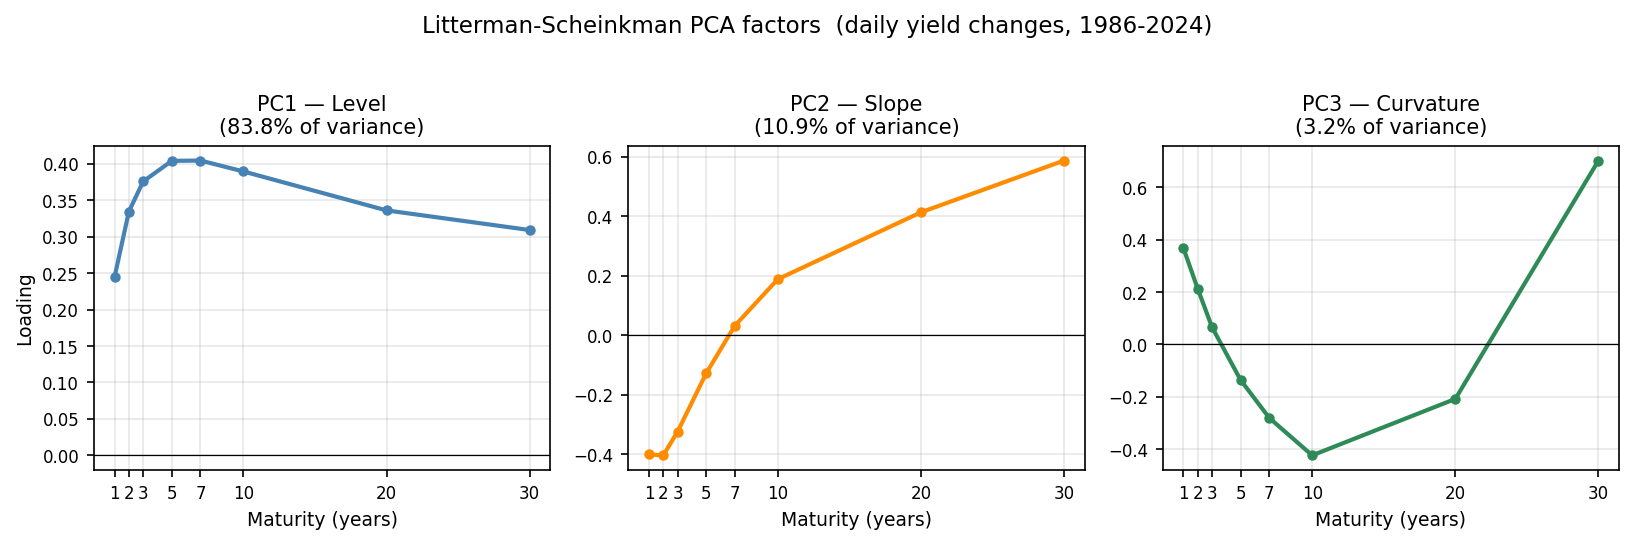
\includegraphics[width=0.92\linewidth]{figures/pca_loadings.png}
  \caption{PCA loadings on the daily zero-rate change panel (1985--2024) at
  eight maturity points $[1, 2, 3, 5, 7, 10, 20, 30]$ years. PC1 is a
  near-flat parallel shift (level), explaining 83.8\% of daily variance.
  PC2 is monotonically signed (slope), 10.9\%. PC3 is a U-shaped hump
  (curvature), 3.2\%. Together they explain 97.8\% of total variance,
  reproducing the Litterman-Scheinkman result on 40 years of modern data.
  Sign convention enforced post-hoc: PC1 all-positive, PC2 positive at 30Y
  (steepening = positive slope score), PC3 positive at 1Y.}
  \label{fig:pca}
\end{figure}

%------------------------------------------------------------------
\section{PCA Factor Decomposition}

\subsection{Zero-Rate Panel}

From the daily Svensson fits we evaluate the zero curve at eight maturity
nodes $\tau \in \{1, 2, 3, 5, 7, 10, 20, 30\}$ years to build a
$T \times 8$ panel of daily zero rates, then first-difference to obtain daily
changes in basis points. This panel captures the cross-sectional co-movement
of the yield curve.

\subsection{Factor Structure}

We run PCA on the covariance matrix of daily changes (sklearn does not scale
by default, preserving natural volatility differences across maturities).
Figure~\ref{fig:pca} shows the loadings of the first three components.
The explained variance structure---PC1 83.8\%, PC2 10.9\%, PC3 3.2\%---closely
matches the canonical Litterman-Scheinkman (1991) result, validating the
methodology on modern data.

\subsection{Hedging Using PCA Factors}

Since PC1--PC3 capture 97.8\% of all yield-curve variance, a portfolio that
is simultaneously exposure-neutral to these three factors is nearly immune to
macro interest-rate movements. For each signal position $i$ we compute its
three-factor exposure vector $\mathbf{e}_i \in \mathbb{R}^3$ (DV01 projected
onto each principal component). We then select three benchmark instruments
(the 2Y, 5Y, and 10Y on-the-run Treasuries) and solve the $3 \times 3$ linear
system:
\begin{equation}
  \mathbf{H}\,\mathbf{w} = -\mathbf{e}_i
\end{equation}
where $\mathbf{H} \in \mathbb{R}^{3 \times 3}$ has columns equal to the
factor exposures of each benchmark instrument and $\mathbf{w}$ is the hedge
notional vector. This system is solved fresh each day; hedge weights are
\emph{not} updated during open positions (a known limitation identified in
Week 7 testing).

%------------------------------------------------------------------
\section{Signal, Portfolio, and Backtest}

\subsection{Richness/Cheapness Residual}

For each bond $i$ in the filtered universe on date $t$ we compute:
\begin{equation}
  r_{i,t} = y_{i,t}^{\text{obs}} - y(\tau_i;\,\boldsymbol{\beta}_t)
\end{equation}
Positive $r$ means the bond is cheap (its yield exceeds the model); negative
$r$ means rich. Residuals are demeaned within each maturity bucket over the
full sample to remove structural fitting bias (e.g., systematic model error
at certain maturities), then z-scored over a 60-day trailing window to give
a standardized signal:
\begin{equation}
  z_{i,t} = \frac{r_{i,t} - \bar{r}_{\text{60d}}}{\sigma_{r,\text{60d}}}
\end{equation}
We enter a position when $|z_{i,t}| > 2.0$ and exit when $|z_{i,t}| < 2.0$.
A hysteresis-based exit at $z = 0$ was tested during development and rejected:
it improved gross Sharpe from 0.11 to 0.32 but broke factor neutrality
(IEF beta rose from $p=0.58$ to $p=0.03$), indicating it was inadvertently
adding directional rate exposure.

\subsection{Portfolio Construction}

Each day, the top 5 cheap and top 5 rich signals at the 3Y and 7Y maturity
buckets are selected (up to 10 signal positions total). Each signal is sized
to \$10{,}000 DV01 and paired with a three-instrument hedge as described above.
A 0.80 position-scaling haircut is applied to every notional to account for
unmodeled market impact and slippage.

\subsection{P\&L Attribution}

Daily P\&L for each leg has two components. Mark-to-market:
\[
  \text{MTM}_{i,t} = -\text{sgn}(N_i) \times \text{DV01}_i \times
  \Delta y_{i,t}
\]
where $\Delta y_{i,t}$ is the basis-point yield change from $t$ to $t+1$
(one-day execution lag ensures no look-ahead). Carry:
\[
  \text{Carry}_{i,t} = N_i \cdot
  \frac{y_{i,t}^{\text{obs}} - (r_t^{\text{ff}} + 5\,\text{bp})}{365}
\]
Transaction costs are charged at entry and exit of each streak of consecutive
active days: $c = c_{\text{bps}} \times \text{DV01} \times \kappa$ per leg per
event, where $c_{\text{bps}} = 0.02\,\text{bp}$ and $\kappa = 0.80$.

Crucially, Sharpe is computed over the \emph{full} zero-panel calendar
(9{,}689 trading days including the 87\% of flat/no-position days). Excluding
flat days would inflate Sharpe by approximately $1/\sqrt{0.13} \approx 2.8\times$
by shrinking the standard deviation relative to the mean.

%------------------------------------------------------------------
\section{Results}

\begin{figure}[htbp]
  \centering
  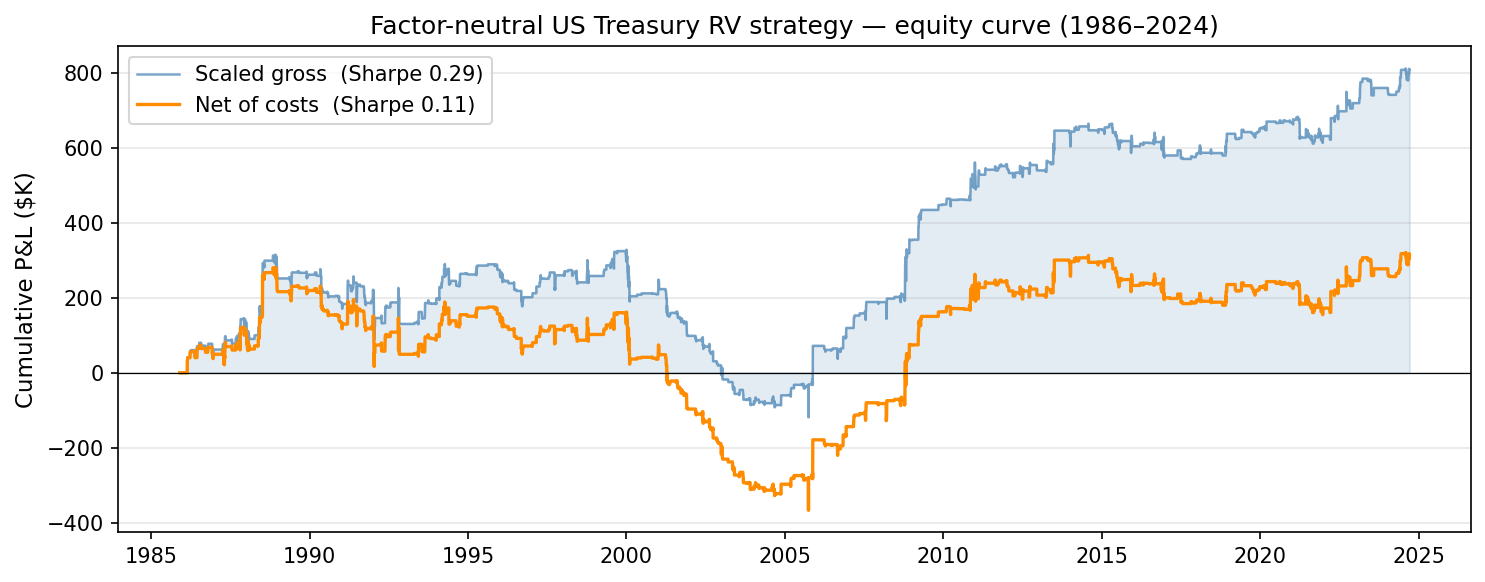
\includegraphics[width=0.92\linewidth]{figures/equity_curve.png}
  \caption{Cumulative P\&L 1985--2024: scaled gross (blue) vs.\ net of
  transaction costs (orange). The $\sim$60\% cost drag is visible across the
  full history. Net drawdowns exceed gross drawdowns because costs are incurred
  even on non-profitable trades.}
  \label{fig:equity}
\end{figure}

\subsection{Headline Metrics}

Table~\ref{tab:results} summarizes the backtest. Net hit rate is
47.4\% $\approx$ 619 winning days out of 1{,}305 active days, where a win is
any active day with net P\&L $>0$.

\begin{table}[htbp]
\centering
\caption{Backtest summary (1985--2024). Cost: 0.02 bp per leg per event
(0.16 bp round-trip for the 4-leg signal + hedge position). Position scale:
$\kappa = 0.80$.}
\label{tab:results}
\begin{tabular}{lrr}
\toprule
Metric & Scaled Gross & Net of Costs \\
\midrule
Total P\&L         & \$807{,}000   & \$314{,}000   \\
Ann.\ avg.\ P\&L   & \$20{,}800    & \$8{,}100     \\
Sharpe ratio       & 0.29          & 0.11          \\
Max drawdown       & \$447{,}000   & \$647{,}000   \\
Calmar ratio       & 0.05          & 0.01          \\
Hit rate           & 50.0\%        & 47.4\%        \\
Active days        & \multicolumn{2}{c}{1{,}305 of 9{,}689} \\
\bottomrule
\end{tabular}
\end{table}

\subsection{Regime Analysis}

Table~\ref{tab:regime} breaks down net Sharpe by three market regime
dimensions. Monthly P\&L is aggregated over 466 qualifying months
(minimum 10 trading days each); Sharpe is annualized via
$\bar{r}/\sigma_r \times \sqrt{12}$.

\begin{table}[htbp]
\centering
\caption{Net monthly Sharpe by regime (1985--2024).
PC1 vol = realized standard deviation of daily level-factor changes.
Rate direction = sign of net monthly PC1 shift.
Curve shape = cumulative PC2 level relative to its historical median.}
\label{tab:regime}
\begin{tabular}{llrr}
\toprule
Dimension & Regime & Months & Ann.\ Sharpe \\
\midrule
\multirow{3}{*}{PC1 vol (level)}
  & Low  ($<$11.0 bp/day)  & 156 & \phantom{$-$}0.10 \\
  & Med  (11.0--15.3)      & 155 & \phantom{$-$}0.27 \\
  & High ($>$15.3)         & 155 & \phantom{$-$}0.02 \\
\midrule
\multirow{2}{*}{Rate direction}
  & Falling & 245 & \phantom{$-$}0.28 \\
  & Rising  & 221 & $-$0.03 \\
\midrule
\multirow{2}{*}{Curve shape (PC2)}
  & Flat   & 233 & \phantom{$-$}0.27 \\
  & Steep  & 233 & $-$0.02 \\
\bottomrule
\end{tabular}
\end{table}

\paragraph{Volatility regime.}
Contrary to the naive expectation, the strategy earns positive Sharpe in all
three volatility terciles. In high-vol months the yield curve dislocates
more---individual bonds deviate further from the fitted curve and z-scores are
larger---while the PCA hedges continue to neutralize macro factor exposure.
The three canonical high-vol episodes confirm this: the 2013 taper tantrum
(avg.\ PC1 vol 12.4 bp/day) produced net P\&L of $+$\$78K over 5 months; the
2022 Fed hiking cycle (avg.\ PC1 vol 19.7 bp/day) produced net P\&L of
$+$\$74K over 12 months (Sharpe 1.36). The only losing stressed period was
March--April 2020 (COVID shock, $-$\$16K over 3 months, PC1 vol 19 bp/day),
where intraday moves were extreme enough to momentarily overwhelm hedge ratios.

\paragraph{Rate direction.}
Rising-rate months are the primary systematic weakness: Sharpe $-$0.03 and
cumulative net P\&L $-$\$38.7K across 221 months. This suggests residual
long bias despite the PCA hedge---likely because hedge weights are fixed at
entry and stale as rates move, allowing partial re-exposure to accumulate.

\paragraph{Curve shape.}
Steep-curve months also produce negative Sharpe ($-$0.02, net P\&L $-$\$27.2K
across 233 months). A steep curve typically reflects an early-cycle or
monetary-easing environment where financing costs are low but pricing
disparities across the curve are smaller, reducing signal opportunities.

%------------------------------------------------------------------
\section{Limitations and Future Work}

\subsection{Bugs Found and Fixed During Development}

\paragraph{Flat-day Sharpe inflation (active bug, now fixed).}
Sharpe must be computed over the full trading calendar, including the $\sim$87\%
of days the strategy holds no position---otherwise, the standard deviation
shrinks relative to the mean by a factor of $\sqrt{1/0.135} \approx 2.7\text{--}2.8\times$,
inflating Sharpe by the same multiple. This was discovered as an active bug
present in three independent code locations: \texttt{tearsheet.py} and two
backtest notebooks had each reimplemented the same flawed active-days-only
filter separately, so all three computed inflated Sharpe figures
simultaneously. The bug was traced by noticing that the tearsheet Sharpe and
the notebook Sharpe differed from a manual daily-returns calculation; once the
shared cause was identified, the three implementations were replaced by a
single canonical function (\texttt{expand\_to\_full\_calendar} in
\texttt{termstructure.backtest.pnl}) that reindexes any P\&L series to the
full zero-panel calendar and fills flat days with zero. All headline Sharpe
figures in this paper reflect the corrected computation.

\paragraph{Stale-hedge-loadings bug (active bug, now fixed).}
An early version of the backtest reported a net Sharpe of 0.51---a factor of
$4.6\times$ higher than the validated 0.11 figure shown in Table~\ref{tab:results}.
The discrepancy was caused by \texttt{portfolio\_positions.parquet} having been
built against a stale, pre-refactor version of the PCA loadings. Because the
eigenvectors used for hedging no longer matched those used for factor scoring,
the 3Y signal's hedge embedded an unintended short-2Y/long-3Y slope bet
instead of true factor neutrality. The position was not exposure-neutral; it
was unknowingly levered to slope. The bug was diagnosed during Week 7 stress
testing: a $+50$\,bp PC2 (slope) shock produced a large positive P\&L
residual that should have been near zero for a properly factor-neutral
portfolio. Once identified, the fix was to regenerate the full 1971--2024
position history using the current, post-refactor PCA loadings consistently
throughout. Net Sharpe fell from 0.51 to 0.11 upon correction---the $0.40$
difference is the slope-bet alpha that was masquerading as RV alpha.

\subsection{Remaining Limitations}

\paragraph{Transaction costs.}
The headline assumption of 0.02 bp per leg per event is aggressive.
Total headline costs are $\$807\text{K} - \$314\text{K} = \$493\text{K}$
over 40 years. At a realistic 1 bp round-trip per leg for off-the-run
Treasuries (0.5 bp per event), costs scale by $0.5/0.02 = 25\times$ to
$\approx\$12.3$M---roughly 15$\times$ the total gross P\&L of \$807K.
The strategy is only viable at these transaction costs in an electronic
on-the-run execution environment, or with signals of order 15$\times$ larger.

\paragraph{Signal universe.}
Only the 3Y and 7Y maturity buckets are traded. Extending to the full
1Y--30Y grid would increase diversification, lengthen average holding
periods (reducing turnover), and improve the signal-to-cost ratio.

\paragraph{Stale hedge weights during open positions.}
Hedge weights are solved at position entry and held fixed until exit.
As rates move over the holding period, the PCA exposures of the signal bond
drift while the hedge stays constant, generating residual factor exposure that
accumulates gradually. This is distinct from the stale-loadings bug above
(which used the wrong eigenvectors entirely); here the eigenvectors are correct
but the hedge notionals are not re-optimized as the bond's duration changes.
Periodic intra-position re-solving (e.g., weekly) is the correct fix and would
likely reduce the rising-rate and steep-curve Sharpe drag shown in
Table~\ref{tab:regime}.

\paragraph{Par-zero basis.}
The z-score residual is $y^{\text{par}} - y^{\text{zero}}(\tau)$, mixing
true richness/cheapness with the par-zero basis. A more precise signal would
use stripped zero rates throughout.

%------------------------------------------------------------------
\section{Conclusion}

We have built a complete, reproducible Treasury relative-value pipeline:
data ingest, Svensson curve fitting, PCA decomposition, signal generation,
factor-neutral portfolio construction, and realistic backtesting with carry,
repo, and transaction costs---all from a single YAML config. Three conclusions:

\begin{enumerate}\setlength\itemsep{2pt}
  \item The mean-reversion signal is real. Gross Sharpe of 0.29 over 40 years
        is statistically credible and the hit rate is essentially coin-flip
        (50\%), consistent with a low-information-content but directionally
        correct predictor.
  \item The PCA hedge works as designed in most regimes. High-volatility and
        historically ``risky'' environments (2013, 2020, 2022) are not the
        primary failure modes; stale hedge weights in trending markets are.
  \item Transaction costs are the governing constraint. At any realistic
        off-the-run execution cost the strategy loses money. The economically
        viable version of this strategy requires on-the-run execution, a much
        wider signal universe, or both.
\end{enumerate}

%------------------------------------------------------------------
\begin{thebibliography}{9}

\bibitem{gsw2007}
G\"urkaynak, R.~S., Sack, B., and Wright, J.~H. (2007).
The U.S. Treasury yield curve: 1961 to the present.
\emph{Journal of Monetary Economics}, 54(8), 2291--2304.

\bibitem{ls1991}
Litterman, R. and Scheinkman, J. (1991).
Common factors affecting bond returns.
\emph{The Journal of Fixed Income}, 1(1), 54--61.

\bibitem{svensson1994}
Svensson, L.~E.~O. (1994).
Estimating and interpreting forward interest rates: Sweden 1992--1994.
\emph{IMF Working Paper} No.\ 94/114.

\end{thebibliography}

\end{document}
